\section{\stSmalltalkConceptsTerm}

\stSmalltalkConceptsDefinition

\subsection{\stSmalltalkSyntaxTerm}

\noindent
\begin{tabularx}{\linewidth}{@{}rX@{}}
	\toprule
	\multicolumn{2}{l}{\stReservedWordsTerm}\\
	\midrule
	\code{nil} & \stNilDefinition\\
	\code{true} \stAndTerm{} \code{false} & \stTrueAndFalseDefinition\\
	\code{self} & \stSelfDefinition\\
	\code{super} & \stSuperDefinition\\
	\code{thisContext} & \stThisContextDefinition\\
	\addlinespace

	\toprule
	\multicolumn{2}{l}{\stReservedCaractersTerm}\\
	\midrule
	\code{:=} (\stOrTerm{} \code{\textleftarrow}) & \stAssignmentOperatorDefinition \\
	\code{\^} (\stOrTerm{} \code{\textuparrow}) & \stReturnOperatorDefinition \\
	\code{|} var1 var2 var3 \code{|} & \stTempsDeclarationOperatorDefinition \\
	\code{\$a} & \stDollarOperatorForCharacterADefinition \\
	\code{\#(abc 123)} & \stLiteralArrayDefinition \\
	\code{.} (\stPeriodTerm) & \stDotOperatorDefinition \\
	\code{;} & \stSemiColonOperatorDefinition \\
	\code{[ ]} & \stBlockOperatorDefinition \\
	\code{"}\stCommentTerm\code{"} & \\
	\code{'}\stStringTerm\code{'} & \\
	\bottomrule
\end{tabularx}

\subsection{\stMessageSendingTerm}

\stMessageSendingDefinition

\paragraph{\stUnaryMessagesTerm}

\stUnaryMessagesDefinition

\paragraph{\stBinaryMessagesTerm}

\stBinaryMessagesDefinition

\paragraph{\stKeywordMessagesTerm}

\stKeywordMessagesDefinition

\subsection{\stBlockTerm}

\stBlockDefinition

\section{\stDevelopmentEnvironmentTerm}

\stDevelopmentEnvironmentDefinition

\begin{center}
  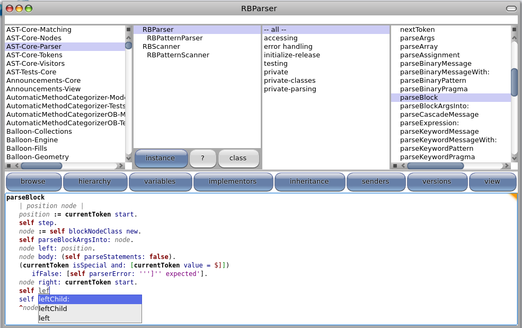
\includegraphics[width=\stSqueakCodeBrowserSize\textwidth]{pharo}\\
  \stSqueakCodeBrowserTerm
\end{center}

%-- MISSING SQUEAK CODE BROWSER PICTURE --

\section{\stImplementationTerm}

\stImplementationDefinition

\pagebreak{}

\section{\stApplicationsTerm}

\stApplicationsDefinition

\begin{center}
  \includegraphics[width=\stApplicationScreenshotPictureWidth\textwidth]
  {\stApplicationScreenshotPicture}\\
  \stApplicationScreenshotTerm
\end{center}

\begin{stGlossary}
\stWordDefinition{Image}
\stWordDefinition{VM}
\stWordDefinition{Reflexion}
\stWordDefinition{DynamicTyping}
\end{stGlossary}

\pagebreak{}

\section{\stBooksTerm}

\stBooksDefinition

\section{\stSmalltalkActionsTerm}

\stSmalltalkActionsDefinition

\section{Internet}

\stInternetWebsitesDefinition

%%% Local Variables: 
%%% mode: latex
%%% TeX-master: "../flyer"
%%% ispell-local-dictionary: "english"
%%% End: 
